\section{Overview}
\begin{itemize}
    \item Up until this point, all data that our prograam accesses is via memory (RAM):
        \begin{itemize}
            \item Scope and variety of applications you can create is limited. 
            \item Using memory goes away when the program goes away.
            \item Specially on embedded systems memory is scarce.
            \item You want to have this ability for reading and writing persistent data on a hard drive. 
        \end{itemize}
    
    \item All serious business applications require more data than would fit into main memory:
        \begin{itemize}
            \item It also depends on the ability to process data that is persistent and stored on an external device such as a disk. 
        \end{itemize}
    
    \item C provides many functions in the header file stdio.h for writing to and reading from external devices.
        \begin{itemize}
            \item The external device you would use for storing and retrieving data is typically a disk drive.
            \item However, the library will work with virtually any external storage device.
        \end{itemize}
    
    \item With all the example up to this point, any data the user enters is lost once the program ends, this is called volatile memory meaning the data is not persistent.
        \begin{itemize}
            \item If the user wants to run the program with the same data, he or she must enter it again each time.
            \item Very inconvenient and limits programming.
            \item Referred to as volatile memory.
        \end{itemize}
\end{itemize}

\subsection{Files}
\begin{itemize}
    \item Programs need to store data on permanent storage:
        \begin{itemize}
            \item This is non-volatile (it stays around).
            \item Continues to be maintained after the computer is turned off.
        \end{itemize}
    
    \item A file can store non-volatile data and is usually stored on a disk or solid-state device:
        \begin{itemize}
            \item A named section of storage.
            \item stdio.h is a file containing useful information.
        \end{itemize}
    
    \item C views a file as a continuous sequence of bytes.
        \begin{itemize}
            \item A file inside a Linux or windows operating system is stored a certain way, but as far as C as a programming language goes, it's just a sequence of bytes.
            \item Each byte can be read individually.
            \item Corresponds to the file structure in the Unix environment.
        \end{itemize}
    
        \begin{figure}[H]
            \centering
            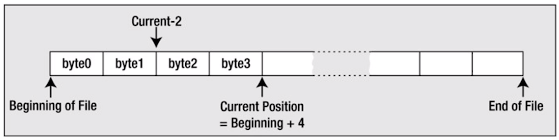
\includegraphics[width=14cm]{\figs/files.png} 
            \caption{Taken from Beginning C,Horton}
        \end{figure}
        
    \item A file has a beginning and an end, as well as a current position (defined as so many bytes from the beginning).
    \item The current position is where any file action (read/write) will take place.
        \begin{itemize}
            \item You can move the current position to any point in the file (even the end).
            \item This is relevant because we want to seek the beginning position to start writing the file, and seek the end to stop.
        \end{itemize}
\end{itemize}

\subsection{Text and binary files}
\begin{itemize}
    \item There are two ways of writing data to a stream that represents a file.
        \begin{itemize}
            \item Text 
            \item Binary
        \end{itemize}

    \item Text data is written as a sequence of characters organized as lines (each line ends with a newline).
        \begin{itemize}
            \item Text data can vary from system to system depending on how the system interprets the bytes, for example on Windows DOS every line has a carriage return (\verb|\r|) and a newline (\verb|\n|) so when you read and write to a file you need to take this in to account.
        \end{itemize}
    
    \item Binary data is written as a series of bytes exactly as they appear in memory.
        \begin{itemize}
            \item Image date, music encoding — non-readable.
            \item These are not readable because they are just bytes, if you were to open them in a text editor you would not see anything you understand.
        \end{itemize}
    
    \item You can write any data you like to a file.
        \begin{itemize}
            \item Once a file has been written, it just consists of a series of bytes.
        \end{itemize}
    
    \item You have to understand the format of the file in order to read it.
        \begin{itemize}
            \item A sequence if 12 bytes in a binary file could be 12 characters, 12 8-bit signed integers, 12 8-bit unsigned integers, etc. This is significant because for example Windows might have extra characters when if writes data. 
            \item In binary mode, each and every byte of the file is accessible. This makes it extra tricky.
        \end{itemize}
\end{itemize}

\subsection{Streams}
\begin{itemize}
    \item A stream:
        \begin{itemize}
            \item Can represent a file, but a stream is a more generic term that can represent any kind of input.
            \item It can represent the keyboard, the console, a file, a socket (if you are using networking).
        \end{itemize}
    
    \item C programs automatically open three files on your behaf:
        \begin{itemize}
            \item Standard input: the normal input device for our system, usually your keyboard.
                \begin{itemize}
                    \item You use this when you do scanf()
                    \item You can actually use scanf() to read from files if you change the input stream.
                \end{itemize}
                
            \item Standard output: usually your display screen. 
                \begin{itemize}
                    \item This is usually via the console.
                \end{itemize}

            \item Standard error: usually also your display screen.
                \begin{itemize}
                    \item You have to redirect it in order to see it.
                \end{itemize}
        \end{itemize}
    
    \item You can also redirect files on the system to be recognized as a standard input output. This is an operating system concept. Sending output to a file is an example of this, get input from a file. 
    \item Standard input is the file that is read by getchar() and scanf().
    \item Standard output is used by putchar(), puts(), and printf().
    \item The purpose of the standard error output file is to provide a logically distinct place to send error messages.
        \begin{itemize}
            \item To access it you need special commands.
        \end{itemize}
    
    \item A stream is an abstract representation of any external source or destination for data.
        \begin{itemize}
            \item The keyboard, the command line on your display, and files on a disk are all examples of things you can work with as streams. This will become even more significant when you program in C++.
            \item The C library provides functions for reading and writing to or from data streams.
                \begin{itemize}
                    \item You use the same input/output functions for reading and writing any external device that is mapped to a stream.
                    \item This is why you can use scanf to read from files. It all depends on which stream we use.
                \end{itemize}
        \end{itemize}
\end{itemize}


%----------------------------------------------------------------------------------------
\section{Accessing files}
\begin{itemize}
    \item Files on disk have a name and the rules for namign files are determined by your operating system.
        \begin{itemize}
            \item You may have to adjust the names depending on what OS your program is running.
        \end{itemize}
    
    \item A program references a file through a file pointer (or stream pointer, since it works on more than a file):
        \begin{itemize}
            \item You associate a file pointer with a fie programmatically when the program is run. You will create a pointer variable of type FILE in your program. We use these file pointers as a more effective way to refer to the file, because the name can cause ambiguity, the pointer will refer to what's actually being pointed to. 
            \item Pointers can be reused to point to different files on different occasions.
            \item A file pointer should really be referred to as a stream pointer.
        \end{itemize}
    
    \item A file pointer points to a struct of type FILE that represents a stream, you can actually look at the struct of type file to see what is inside it.
        \begin{itemize}
            \item Contains information about the file:
                \begin{itemize}
                    \item Whether you want to read or write or update the file.
                    \item The addresses of the buffer in memory to be sued for data.
                    \item A pointer to the current position in the file for the next operation.
                \end{itemize}
            
            \item The above is all set via input/output file operations.
                \begin{itemize}
                    \item When you open a file it needs to know if it's a binary or a text file, so that methods such as seek adapt to the file type.
                \end{itemize}
        \end{itemize}
    
    \item If you want to use several files simultaneously in a program, you need a separate file pointer for each file.
        \begin{itemize}
            \item There is a limit to the number of files you can have open at one time.
                \begin{itemize}
                    \item Defined as FOPEN\_MAX in stdio.h.
                    \item It depends as well on the operating system you are running on.
                \end{itemize}
            
            \item It's not a good idea to have more than one file opened if it's not absolutely necessary, files are saved in persistent memory and copying all of that from persistent memory to RAM takes more time and can make you programs unresponsive.
            \item You can only reuse a pointer if you are reading or writing at different times.
        \end{itemize}
\end{itemize}

\subsection{Open name}
\begin{itemize}
    \item You can associate a specific external file name with an internal file pointer variable though a process refered to as opening a file.
        \begin{itemize}
            \item Via the \mintinline{c}{fopen()} function:
                \begin{itemize}
                    \item This function returns the file pointer for specific external file.
                \end{itemize}
            \end{itemize}
    
    \item The fopen() function is defined in stdio.h
        \mint{c}{FILE *fopen(const char * restrict name, const char * restrict mode);}
        \begin{itemize}
            \item This is usually your first operation while writing and reading files.
        \end{itemize}
    
    \item The function fopen() takes as a first argument a pointer to a string that is the name of the external file you want to process.
        \begin{itemize}
            \item You can specify the name explicitly or use a char pointer that contains the address of the character string that defines the file name. 
            \item You can obtain the file name through the command line, as input from the user, or defined as constant in you program.
        \end{itemize}
    
    \item The second argument to the fopen() function is a character string that represents the file mode.
        \begin{itemize}
            \item Specifies what to do with the file.
            \item A file mode specification is a character string between double quotes.     
        \end{itemize}
    
    \item Assuming the call to fopen() is successful, the function returns a pointer of type FILE* that you can use to reference the file in further input/output operations using other functions in the library.
    \item If the file cannot be opened for some reason, fopen() returns NULL.
        \begin{itemize}
            \item Just like with malloc, check for NULL in files.
        \end{itemize}
    
    \item The second parameter can follow any of the following conventions.
        \begin{center}
            \begin{tabular}{ |p{5cm}|p{10cm}| }
                \hline
                    Mode & Description \\
                \hline
                    \mintinline{c}{"w"}   & Open a text file for \emph{write} operations. If the file exists, its current contents are discarded. \\
                \hline 
                    \mintinline{c}{"a"}   & Open a text file for \emph{append} operations. All writes are to the end of the file. \\ 
                \hline
                    \mintinline{c}{"r"}   & Open a text file for read operations. \\ 
                \hline
                \multicolumn{2}{|c|}{Adding a + to the option adds the feature of creating the file if it doesn't exist, except for the r.} \\
                \hline
                    \mintinline{c}{"w+"}  & Open a text file for update (reading and writing), first truncating the file to zero lenght if it exists or creating the file if it doesn't exist. \\ 
                \hline
                    \mintinline{c}{"a+"}  & Open a text file for update (reading and writing) appending to the end of the existing file, or creating the file if it doesn't yet exists. \\ 
                \hline
                    \mintinline{c}{"r+"}  & Open a text file for update (for both reading and writing). \\ 
                \hline
            \end{tabular}
        \end{center}
\end{itemize}

\subsection{Write mode}
\begin{itemize}
    \item If you want to write an existing text file with the name myfile.txt
        \begin{minted}[autogobble]{c}
            FILE *pfile = NULL;
            char *filename = "myfile.text";
            pfile = fopen(filename,"w"); // open myfile.txt to write it
            if (pfile == NULL)
                printf("Failed to open %s",filename);
        \end{minted}
    
    \item Opens the file and associates the file with the name myfile.txt with your file pointer pfile:
        \begin{itemize}
            \item The mode as ``w'' means you can only write to the file.
            \item You cannot read it.
        \end{itemize}
    
    \item If a file with the name myfile.txt does not exist, the call to fopen() will create a new file with this name.
    \item If you only provide the file name without any path specification, the file is assumed to be in the current directory:
        \begin{itemize}
            \item You can also specify a string that is the full path and name for the file.
            \item If you want to access a file somewhere else, you have to specify the entire directory, also called the absolute path. Just having the name is called a relative path. 
            \item Relative paths are better because its not dependent on a specified file. You can also move backwards in directories using ``../''. In absolute path is usually like ``\verb|C:\User...|'' and if you ever moved that file your program wouldn't be able to open it.
        \end{itemize}
    
    \item On opening a file for writing, the file length is truncated to zero and the position will be at the beginning of any existing data for the first operation.
        \begin{itemize}
            \item Any data that was previously written to the file will be lost and overwritten by any write operations.
            \item Without providing a + you can only do one operation, reading or writing but not both.
        \end{itemize}
\end{itemize}

\subsection{Append mode}
\begin{itemize}
    \item If you want to add to an existing text file rather than overwrite it:
        \begin{itemize}
            \item Specify mode ``a''.
            \item The append mode operation. 
        \end{itemize}
    
    \item This positions the file at the end of any previously written data.
        \begin{itemize}
            \item If the file does not exist, a new will be created.
        \end{itemize}
        \mint{c}{pFile = fopen("myfile.txt","a"); // Open myfile.txt to add to it}
    
    \item Do not forget that you should test the return value for null each time you use it.
    \item When you open a file in append mode:
        \begin{itemize}
            \item All write operations will be at the end of the data in the file on each write operation.
            \item All write operations append data to the file and you cannot update the existing contents in this mode, it's all at the end.    
        \end{itemize}
\end{itemize}

\subsection{Read mode}
\begin{itemize}
    \item If you want to read a file:
        \begin{itemize}
            \item Open it with mode argument as ``r''.
            \item You can not write to this file.
        \end{itemize}
        \mint{c}{pFile = fopen("myfile.txt","r");}
    
    \item This positions the file to the beginning of the data.
    \item If you are going to read the file:
        \begin{itemize}
            \item If must already exist, there is no point on reading an empty file.
        \end{itemize}
    
    \item If you try to open a file for reading and it doesn't exist, fopen() will return a NULL pointer.
    \item You always want to check the value returned from fopen(). 
\end{itemize}

\subsection{Renaming a file}
\begin{itemize}
    \item Renaming a file is very easy.
        \begin{itemize}
            \item Use the rename() function.
            \item It takes two parameters, pointers of the old name and new name.
        \end{itemize}
        \mint{c}{int rename(const char *oldname, const har *newname);}
    
    \item The integer that is returned will be 0 if the name change was successful and nonzero otherwise.
    \item The file must not be opened when you call rename(), otherwise the operation will fail.
        \begin{minted}[autogobble]{c}
            if (rename("C:\\temp\\myfile.txt","C:\\temp\\myfile_copy.txt")){
                printf("Failed to rename file.");
            } else {
                printf("File renamed successfully.");
            }
        \end{minted}
        \begin{itemize}
            \item You know it's a Windows directory because of the \verb|C:\\|.
            \item Also in order to provide \verb|\| in C, you must provide two, this is because the backslash is used for special escape sequences, thus you need to escape the backslash itself with another one as so: \verb|\\|
        \end{itemize}
    
    \item This will change the name of myfile.txt in the temp directory on drive C to myfile\_copy.txt.
    \item If the file path is incorrect or the file does not exist, the renaming operation will fail.
\end{itemize}

\subsection{Closing a file}
\begin{itemize}
    \item When you have finished with a file, you need to tell the operating system so that it can free up the file:
        \begin{itemize}
            \item You can use it by the fclose() function.
            \item Remember there is a limit to how many files you can have opened at a time. 
        \end{itemize}
    
    \item fclose() accepts a file pointer as an argument.
        \begin{itemize}
            \item Returns EOF (int) of an error occurs.
                \begin{itemize}
                    \item EOF is a special character called the end-of-file character.
                    \item Defined in stdio.h as a negative integer that is usually equivalent to the value -1.
                \end{itemize}
            
            \item 0 if successful.
        \end{itemize}
        \begin{minted}[autogobble]{c}
            fclose(pfile); // Close the file associated with pfile.
            pfile = NULL;
        \end{minted}
    
    \item The result of calling fclose() is that the connection between the pointer, pfile, and the physical file is broken.
        \begin{itemize}
            \item pfile can no longer be used to access the file.
        \end{itemize}
    
    \item If the file was being written, the current contents of the output buffer are written to the file to ensure that the data is not lost. So you don't have to worry about your data, it will be written even if you call the fclose() while it's being written, it will write it first and then close it. 
        \begin{itemize}
            \item This is called thread safe, meaning multiple points of execution in your program.
            \item This process is thread safe because even if another thread is writing your file, fclose() will not close it until the other thread is finished.
        \end{itemize}
    
    \item It is good programming practice to close a file as soon as you have finished with it.
        \begin{itemize}
            \item This protects against output data loss.
        \end{itemize}
    
    \item You must also close a file before attempting to rename it or remove it.
\end{itemize}

\subsection{Deleting a file}
\begin{itemize}
    \item You can delete a file by invoking the remove() function:
        \begin{itemize}
            \item Declared in stdio.h
            \item Just like all the other ones.
        \end{itemize}
        \mint{c}{remove("myfile.txt");}
    
    \item Will delete the file that has the name myfile.txt from the current directory.
    \item The file must be closed in order for this operation to work.
    \item The file cannot be open when you try to delete it, just like rename. 
    \item You should always double check with operations that delete files.
        \begin{itemize}
            \item You could wreck your system if you do not.
            \item Deleting files can cause problems so be careful.
        \end{itemize}
    
    \item Everything is based on that file pointer.
\end{itemize}


%----------------------------------------------------------------------------------------
\section{Reading for a file}
\subsection{Reading characters from a text file}
\begin{itemize}
    \item The fgetc() function reads a character from a text file that has been opened for reading.
        \begin{itemize}
            \item We need to open the file first using the ``r'' or ``r+'' mode.
        \end{itemize}

    \item Takes a file pointer as its only argument and returns the character read as type int.
        \mint{c}{int mchar = fgetc(pfile); // Reads a character into mchar with pfile a File pointer}
    
    \item The mchar is type int because EOF will be returned if the end of the file has been reached.
    \item The function getc(), which is equivalent to fgetc(), is also available.
        \begin{itemize}
            \item Requires an argument of type FILE* and returns the character read as type int.
            \item Virtually identical to fgetc().
            \item Only difference between them is that getc() may be implemented as a macro, whereas fgetc() is a function.
            \item fgetc() has more protection in it. 
        \end{itemize}
    
    \item You can read the contents of a file again when necessary.
        \begin{itemize}
            \item The rewind() function positions the file that is specified by the file pointer argument at the begining.
        \end{itemize}
    
        \inputcode{c}{\code/reading_files.c}
\end{itemize}

\subsection{Reading a string from a text file}
\begin{itemize}
    \item You can use the fgets() function to read from any file or stream.
        \mint{c}{char *fgets(char *str, int nchars, FILE *stream);}
    
    \item The function reads a string into memory area pointed by str, from the file specified by the stream.
        \begin{itemize}
            \item Characters are read until either a \verb|'\n'| is read or nchars-1 characters have been read from the stream, whichever occurs first.
            \item I a newline character is read, it's retained in the string.
                \begin{itemize}
                    \item a \verb|\0| character will be appended to the end of the string.
                \end{itemize}
            
            \item If there is no error, fgets() returns the pointer, str.
            \item If there is an error, NULL is returned.
            \item Reading EOF causes NULL to be returned.
        \end{itemize}
    \inputcode{c}{\code/reading_files_str.c}
\end{itemize}

\subsection{Reading formatted input from a file}
\begin{itemize}
    \item You can get formatted input from a file by using the standard fscanf() function.
        \mint{c}{int fscanf(FILE *stream, const char *format, ...);}
        \begin{itemize}
            \item This is formatted input, formatted input is data that follows some convention such as character delimiters.
        \end{itemize}

    \item The first argument to this function is the pointer to a FILE object that identifies the stream.
    \item The second argument to this function is the format:
        \begin{itemize}
            \item A C string that contains one or more of the following items.
                \begin{itemize}
                    \item White space character.
                    \item Non-white spate character.
                    \item Format specifiers.
                    \item Usage is similar to scanf, but, from a file.
                \end{itemize}
        \end{itemize}
    
    \item The function returns the number of input items successfully matched and assigned.

    \inputcode{c}{\code/file_r_w_fscanf.c}
\end{itemize}


%----------------------------------------------------------------------------------------
\section{Writing to a file}
\begin{itemize}
    \item The simplest write operations is provided by the function fputc().
        \begin{itemize}
            \item Writes a single character to a text file.
        \end{itemize}
        \mint{c}{int fputc(int ch, FILE *pfile);}
    
    \item The function writes the character specified by the first argument to the file identified by the second argument (file pointer)
        \begin{itemize}
            \item Returns the character that was written if successful.
            \item Return EOF of failure.
        \end{itemize}
    
    \item In practice, characters are not usually written to a physical file one by one:
        \begin{itemize}
            \item This is extremely ineficient.
        \end{itemize}
    
    \item The potc() function is equivalent to fputc():
        \begin{itemize}
            \item Requires the same arguments and the return type is the same.
            \item Difference between them is that putc() may be implemented in the standard library as a macro, whereas fputc() is a function.
        \end{itemize}
    \inputcode{c}{\code/writing_chars_file.c}
\end{itemize}

\subsection{Writing a string to a file}
\begin{itemize}
    \item You can use the fputs() function to write to any file stream, it similar to the fgets().
        \mint{c}{int fputs(const char *str, FILE *pfile);}
    
    \item The first argument is a pointer to the character string that is to be written to the file.
    \item The second argument is the file pointer.
    \item This function will write characters from a string until it reaches the \verb|\0| character.
        \begin{itemize}
            \item Does not write the null terminator character to the file.
                \begin{itemize}
                    \item Can complicate reading back variable-lenght strings from a file that have been written by fputs().
                    \item Expecting to write a line of text that has a newline character at the end. 
                    \item You need to explicitly add the null terminator to the file.
                \end{itemize}
        \end{itemize}
    
    \item This function tends to be more eficient than fputc() in writing strings.
    \inputcode{c}{\code/write_str_to_file.c}
\end{itemize}

\subsection{Writing formatted output to a file}
\begin{itemize}
    \item The standard function for formatted output to a stream is fprint().
        \mint{c}{int fprintf(FILE *stream, const char *format, ...);}
    
    \item The first argument to this function is the pointer to a FILE object that identifies the stream.
    \item The second argument to this function is the format:
        \begin{itemize}
            \item A C string that contains one or more of the following items.
                \begin{itemize}
                    \item White space character.
                    \item Non-white space character.
                    \item Format specifiers.
                    \item Usage is similar to printf, but to a file.
                \end{itemize}
        \end{itemize}
    
    \item If successful, the total number of characters written is returned otherwise, a negative number is returned.
    
    \inputcode{c}{\code/formated_str_to_file.c}
\end{itemize}


%----------------------------------------------------------------------------------------
\section{Finding your position in a file}
\begin{itemize}
    \item File positioning, for many applications, you need to access data in a file other than sequential order (meaning starting in the beginning and ending at the end, byte by byte).
        \begin{itemize}
            \item You might need to go to the middle of the file for example.
        \end{itemize}
    
    \item There are various functions that you can use to access data in random sequence.
    \item There are two aspects to file positioning:
        \begin{enumerate}
            \item Finding out where you are in a file.
            \item Moving to a given point in a file. 
        \end{enumerate}
    
    \item You can access a file at a random position regardless whether you opened the file.
\end{itemize}

\subsection{Finding out where you are, ftell()}
\begin{itemize}
    \item You have two functions to tell you where you are in a file.
        \begin{itemize}
            \item ftell() 
            \item fgetpos()
        \end{itemize}
        \mint{c}{long ftell(File *pfile);}
    
    \item This function accepts a file pointer as an argument and returns a long integer value that specifies the current position in the file.
        \mint{c}{long fpos = ftell(pfile);}
    
    \item The fpos variable now holds the current position in the file and you can use this to return to this position at any subsequent time.
        \begin{itemize}
            \item Value is the offset in bytes from the beginning of the file.
            \item Basically how many bytes from the beginning of the file.
        \end{itemize}
    
        \inputcode{c}{\code/ftell_pos.c}
\end{itemize}

\subsection{fgetpos()}
\begin{itemize}
    \item The second function providing information on the current file position is a little more complicated.
        \mint{c}{int fgetpos(FILE *pfile, fpos_t * position);}
    
    \item The first parameter is a file pointer.
    \item The second parameter is a pointer to a type that is defined in stdio.h:
        \begin{itemize}
            \item fpos\_t: a type that is able to record every position within a file.
        \end{itemize}
    
    \item The fgetpos() function is designed to be used with the positioning function fsetpos().
    \item The fgetpos() function stores the current position and file state information for the file in position and returns 0 if the operation is successful.
        \begin{itemize}
            \item Returns a non-zero integer value for failure.
        \end{itemize}
        \begin{minted}[autogobble]{c}
            fpos_t here;
            fgetpos(pfile,&here);
        \end{minted}
    
    \item The above records the current file position in the variable here.
    \item You must declare a variable of type fpos\_t.
        \begin{itemize}
            \item You cannot declare a pointer of type fpos\_t because there will not be any memory allocated to store the position data.
        \end{itemize}
    
    \inputcode{c}{\code/fgetpos_file.c}
\end{itemize}

\subsection{Setting a position in a file}
\begin{itemize}
    \item As a complement to ftell(), you also have fseek() function.
        \mint{c}{int fseek(FILE *pfile, long offset, int origin);}
    
    \item The first parameter is a pointer to the file you are repositioning.
    \item The second and third parameter define where you want to go in the file. 
        \begin{itemize}
            \item The second parameter is an offset from a reference point specified by the third parameter. 
            \item Reference point can be one of three values that are specified by the predefined names.
                \begin{itemize}
                    \item SEEK\_SET: defines the beggining of a file. 
                    \item SEEK\_CUR: defines the current position in the file.
                    \item SEEK\_END: defines the end of the file.
                \end{itemize}
        \end{itemize}
    
    \item For a text mode file, the second argument must be a value returned by ftell().
    \item The third argument for text mode files must be SEEK\_SET.
        \begin{itemize}
            \item For text files, all operations with fseek() are performed with reference to the beggining of the file. 
            \item For binary files, the offset argument is simple a relative byte count. 
                \begin{itemize}
                    \item Can therefore supply positive or negative values for the offset when the reference point is specified as SEEK\_CUR
                \end{itemize}
        \end{itemize}
    \inputcode{c}{\code/fseek_files.c}
\end{itemize}

\subsection{fsetpos()}
\begin{itemize}
    \item You have the fsetpos() function to go with fgetpos().
        \mint{c}{int fsetpos(FILE *pfile, const fpos_t * position);}
    
    \item The first parameter is a pointer to the open file.
    \item The second is a pointer of the fpos\_t type.
        \begin{itemize}
            \item The position that is stored at the address was obtained by calling fgetpos().
        \end{itemize}
        \mint{c}{fsetpos(pfile, &here);}

    \item The variable here was previously set by a call to fgetpos().
    \item The fsetpos() returns a non-zero value on error or0 when it succeeds.
    \item This function is designed to work with a value that is returned by fgetpos():
        \begin{itemize}
            \item You can only use it to get to a place in a file that you have been before.
            \item fseek() allows you to do to any position just by specifying the appropriate offset.
        \end{itemize}
    
    \inputcode{c}{\code/fgetpos_fsetpos.c}
\end{itemize}

\subsection{Interesting insights}
\begin{itemize}
    \item Whenever you seek for a byte using fseek() using a negative number such as \mintinline{c}{fseek(fp,-10,SEEK_END);} you are really referring to the following procidure.
        \[
            \text{ byte in question (second param)} = \text{ total number of bytes } + (\text{ specified number }) 
        \]
        Thus in the above example we would have: (assuming 812 bytes as total number of bytes)
        \begin{center}
           \begin{align*}
                \text{ byte in question (second param) } &= 812 + (-10) \\ 
                &= 802 \\ 
           \end{align*}
        \end{center}
\end{itemize}


%----------------------------------------------------------------------------------------
\section{Challenge — Find the number of lines in a file}
\inputcode{c}{\code/challenge_num_lines_in_file.c}
\inputcode{c}{\code/challenge_upper_in_file.c}
\inputcode{c}{\code/challenge_files_reverse_order.c}
